\documentclass[12pt]{article}

\usepackage[bottom = 15mm]{geometry}
\usepackage[utf8]{inputenc}
\usepackage[T2A]{fontenc}
\usepackage[russian]{babel}
\usepackage{graphicx}
\usepackage{float}
\usepackage{caption}
\usepackage{amssymb, gensymb, amsmath}
\usepackage{mathrsfs}
\usepackage{array, colortbl}
\usepackage{multicol}


\textwidth = 16 cm
\textheight = 23  cm
\oddsidemargin = 0 pt
\topmargin = -1.5 cm
\parindent = 20 pt
\parskip = 0 pt
\flushbottom


\title{{\bf Задача 4.\,2.\,2 \\ Интерферометр Жамена}}
\author{Лось Денис (группа 611)}
\date{20 мая 2018}

\begin{document}

\maketitle

\paragraph*{Цель работы: } знакомство с техникой интерференционных измерений показателей преломления газов с помощью интерферометра Жамена, настройстка и калиброка интерферометра, исследование смещения интерференционных полос при изменении давления воздуха в одной из камер, при заполнении одной из камер углекислым газом при атмосферном давлении, рассчёт показателей преломления воздуха и углекислого газа при нормальных условиях и средней поляризуемости воздуха.

\paragraph*{В работе используются: } интерферометр Жамена, газовая кювеа, осветитель, зрительная труба, сильфон, баллон с углекислым газом, манометр, краны, светофильтр.

\section*{Экспериментальная установка}
\par
	Схема экспериментальной установик приведена на рисунке 1.
\begin{figure}[h!]
	\centering
	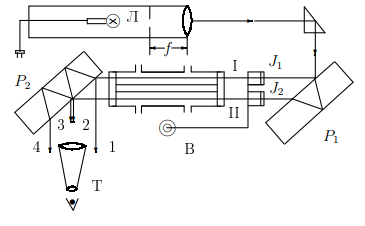
\includegraphics[width = 10cm, height = 5cm]{image1.png}
	\caption{Схема экспериментальной установки}
\end{figure}
\par
	В интерферометре свет от лампы накаливания Л проходит коллиматорный объектив, поворотную призму и слегка расходящимся пучком падает на пластинку $P_1$ под углом $45 \degree$ к ней. Пластины $P_1$ и $P_2$ закреплены на панели, ниже которой имеются два установочных винта. 
\par
	Между пластинами на пути лучей I и II расположена кювета длины $l$, состоящая из двух одинаковых камер, закрытых с торцов плоскопараллельными стеклянными пластинками.
\par
	В одну из камер вводится исследуемый газ, а вторая заполнена воздухом при атмосферном давлении. При этом разность хода $\Delta$, вызванная разностью показателей преломления газом $\delta n$ приводит к сдвигу интерференционных полос:
\[
	\Delta = \delta n \cdot l.
\]
\par
	Сдвиг на одну полосу соответсвует дополнительной разности хода $\Delta = \lambda$. Определив число полос $m$, на которое сместилась картина, можно рассчитать
\[
	\delta n = \frac{\Delta}{l} = m \cdot \frac{\lambda}{l}.
\]
\par
	На пути I и II расположен компенсатор Жамена, состоящий из двух одинаковых плоскопараллельных стеклянных пластинок $J_1$ и $J_2$. Если обе пластинки установлены под одинаковым углом к лучам, то и оптическая длина пути для них для обоих лучей оказывается одинаковой. Поворот одной из пластинок вокруг горизонтальной оси вызывает увеличение или умнеьшение оптической длины пути соответсвующего луча. Это позволяет скомпенсировать разность хода, возникающую в камерах. Для точного отсчёта поворота одна из пластинок снабжена рычагом, конец которого смещается при помощи микрометрического винта В. Пластинки компенсатора ставятся под углом $45 \degree$ к горизонтали, что позволяет использовать линейную экстраполяцию при измерениях. Смещение полос можно наблюдать через трубу $T$.
\par
	Интерферометр Жамена можно применять для измерения небольших изменений преломления жидкостей или газов, а также для определения примесей различных газов в воздухе.
\par
	Показатель преломления исследуемого газа определяется путём сравнения с воздухом при атмосферном давлении:
\[
		n = n_\text{возд} + \frac{\Delta}{l}
\]
\par
	Для определения величины $\Delta$ компенсатор следует прокалибровать.

\section*{Теоритическая часть: зависимость показателя преломления газа от давлениях и температуры}
\par
	Соотношение между показателем преломления газа и его плотностью:
\begin{equation}
	n = \sqrt{\varepsilon} = \sqrt{1 + 4 \pi N \alpha} \approx 1 + 2 \pi N \alpha,
\end{equation}
где $N$ --- число молекул в единице объёма, $\alpha$ --- поляризуемость молекулы.
\par
	Принимая во внимание соотношение $P = N k_\text{б} T$, где $P$ --- давление в газе,  получим
\[
	n - 1 = 2 \pi \alpha \frac{P}{k_\text{б} T}
\]
\par
	Отсюда следует, что при постоянной температуре изменение показателя преломления $\Delta n$ пропорционально изменению давления $\Delta P$:
\[
	\delta n = \frac{2 \pi \alpha}{k_\text{б} T} \Delta P \quad (\text{CГС})
\]
\par
	Величина $\delta n$ измеряется с помощью интерферометра Жамена, $\Delta P$ --- с помощью манометра. Одновременно измерение этих величин (и температуры $T$) позволяет определить поляризуемость молекул воздуха и, следовательно, рассчитать, показатель преломления воздуха при любых значениях $P$ и $T$. Так как воздух является смесью газов, то под поляризуемостью молекул воздуха нужно понимать некоторую среднюю величину, определяемую соотношением
\[
	\alpha = \frac{1}{N} \sum_i \alpha_i N_i
\]
\par
	Установим связь показателя преломления газа $n$ при температуре $T$ и давлении $P$ с показателем преломления $n_0$ при нормальных условиях $(T_0 = 273 \, \text{К}, P_0 = 1 \, \text{атм})$:
\[
	\frac{n_0 - 1}{n - 1} = \frac{T}{T_0} \frac{P_0}{P}
\]

\section*{Параметры экспериментальной установки}
\par
	Длина кюветы $l = 10$ см. Полоса пропускания светофильтра $\lambda = 630 : 670$ нм, длина волны $\lambda_0 = 650$ нм. Давление в помещении $P = (100700 \pm 100)$ Па, температура $T = (25.6 \pm 0.2) \, \degree C$.
\newpage
\section*{Калибровка компенсатора и построение калибровочного графика}
\par
	Приведём результаты отсчёта по компенсатору $z_m$ от номера освещённой полосы $m$.
\begin{table}[h!]
	\centering
	\begin{tabular}{|c|c|}
	\hline
		$m$ & $z_m$, мм \\
	\hline
		-4 & 15.18 \\
	\hline
		-3 & 15.23 \\
	\hline
		-2 & 15.28 \\
	\hline
		-1 & 15.34 \\
	\hline
		0 & 15.38 \\
	\hline
		1 & 15.42 \\
	\hline
		2 & 15.48 \\
	\hline
		3 & 15.54 \\
	\hline
		4 & 15.60 \\
	\hline
		5 & 15.65 \\
	\hline
		6 & 15.70 \\
	\hline
		7 & 15.76 \\ 
	\hline
	\end{tabular}	
\end{table}
\par
	Построим калибровочный график $z = f(m)$.
\begin{figure}[h!]
	\centering
	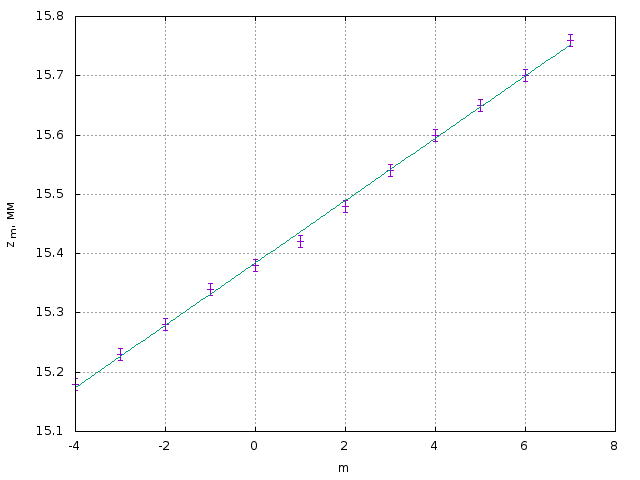
\includegraphics[width = 10cm, height = 5cm]{plot1.png}
	\caption{График зависимости $z = f(m)$}
\end{figure}
\par
	Коэффициент наклона графика
\[
	\beta = \left(0.0526 \pm 0.0007 \right) \, \text{мм}
\]
\par
	Тогда разность хода $\Delta$
\[
	\Delta = \frac{z}{\beta} \lambda_0
\]

\section*{Определение показателя преломления воздуха в условиях опыта и средней поляризуемости молекулы воздуха}
\par
	Изменяя давление с помощью сильфона и совмещая нулевую полосу с перекрестием, снимем зависимость показаний компенсатора $z$ от перепада давлений $\Delta P$. Построим график $z = f(\Delta P)$
	
\begin{table}[h!]
	\centering
	\begin{tabular}{|c|c|}
	\hline
		$z$, мм & $\Delta P$, мм H20 \\
	\hline
		16.38 & 100 \\
	\hline
		16.32 & 200 \\
	\hline
		16.28 & 400 \\
	\hline
		16.24 & 600 \\
	\hline
		16.21 & 700 \\
	\hline
	\end{tabular}
\end{table}

\begin{figure}[h!]
	\centering
	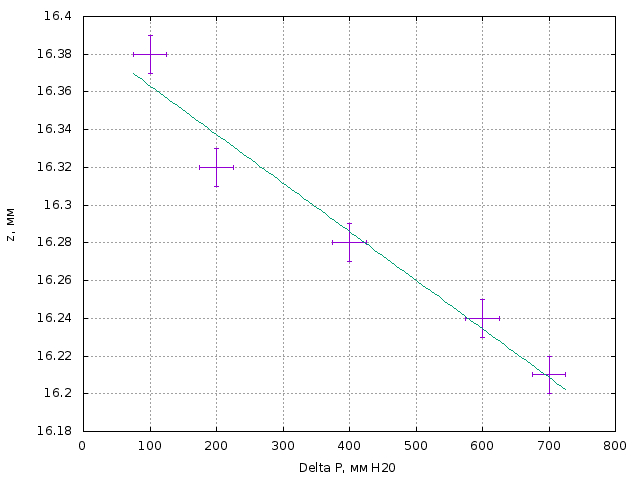
\includegraphics[width = 10cm, height = 5cm]{plot2.png}
\end{figure}
\par
	Коэффициент наклона графика
\[
	\gamma = \left(26 \pm 3 \right) \cdot 10^{-5} \, \frac{\text{мм}}{\text{мм H20}}
\]
\par
	В итоге
\[
	\gamma = \frac{2 \pi \alpha}{k_\text{б} T} \frac{\beta l}{\lambda_0}
\]
\par
	Рассчитаем среднюю поляризуемость молекулы воздуха $\alpha$
\[
	\alpha = \frac{k_\text{б} T}{2 \pi} \frac{\lambda_0 \gamma}{\beta l}
\]
\par
	Средняя поляризуемость молекулы воздуха
\[
	\alpha = \left(2.15 \pm 0.12 \right) \cdot 10^{-30} \text{}
\]
\par
	Показатель преломления воздуха (в условиях опыта)
\[
	n = \left(1.00 \pm 0.06 \right)
\]
\par
	Показатель преломления воздуха (в нормальных условиях)(из-за погрешности не видем разницу)
\[
	n = \left(1.00 \pm 0.06 \right) 
\]

\section*{Оценка радиуса молекулы азота}
\par
\[
	\alpha \approx r^3
\]
где $r$ --- радиус молекулы азота, а значит,
\[
	r \approx 0.13 \, \text{нм}
\]
\par
	Тогда как табличное значение $r = 0.16$ нм.

\section*{Определение показателя преломления углекислого газа}	
\par
	В результате измерений мы получаем отличие от показателя преломления воздуха на 0.00008, однако погрешность, с которой мы определили показатель преломления воздуха, не позволяет нам точно определить значение показателя преломления углекислого газа.

\section*{Выводы}
\par
	В результате работы мы определили среднюю поляризуемость молекулы воздуха, а также показатель преломления воздуха в условиях опыта, а также при нормальных условиях. Однако последующей обработке результатов мешает тот факт, что в ходе исследования зависимости показаний компенсатора от перепада давлений, были получены значения, которые плохо экстраполируются графиком линейной функции. Именно из-за этого определить точно показатель преломления углекислого газа не представляется возможным (т.е. получить отличие от показателя преломления воздуха). Однако в ходе работы мы познакомились с устройством интерферометра Жамена, а также смогли провести оценку радиуса молекулы азота.
\end{document}